\section{Avaliação de ruído e consistência}
\label{sec:teste-ruido}

Para entender o ambiente onde a aplicação foi desenvolvida e testada no âmbito
de ruído e pontos de referência Wi-Fi foi executada uma captura de referência
durante a noite quando ninguém habitava o prédio prototipo portanto nenhum
dispositivo foi movimentado até a manhã seguinte.

Nesta captura dois sensores foram utilizados posicionados a menos de 10
centímetros de distância um do outro sobre uma mesa a um metro do chão no ponto
azul de legenda \emph{'sensor 2'} idicado na \autoref{fig-planta-baixa}. A captura
ocorreu de \emph{2:50} até aproximadamente \emph{11:25} totalizando aproximadamente 8 horas de
captura.

\begin{figure}[htb]
	\caption{\label{fig-planta-baixa}Ambiente de teste}
	\begin{center}
		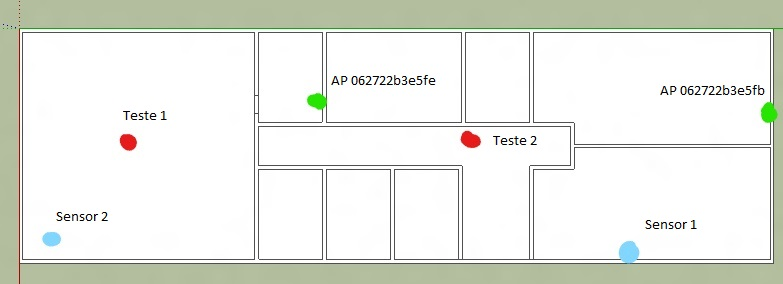
\includegraphics[width=1\textwidth]{060-testes/data-analisis/planta-baixa_Ink_LI.jpg}
	\end{center}
	\legend{Fonte: Elaborada pelo autor}
	\nota[Em azul]{Sensores da aplicação}%
	\nota[Em verde]{Pontos de acesso da rede Wi-Fi do laboratório}%
	\nota[Em verbelho]{Pontos do dispositivo teste}%
\end{figure}


Para o primeiro sensor o sumário indicou que foram capturados \emph{1 729 624}
pacotes num arquivo de \emph{155 MB} com \emph{88} transmissores únicos.
Para o segundo sensor o sumário indicou que foram capturados \emph{1 554 319}
pacotes num arquivo de \emph{134 MB} com \emph{66} transmissores únicos.
Em ambos os sensores se destacaram dois endereços MAC que são os pontos de
acesso para rede Wi-Fi do laboratório.

Os pacotes capturados dos pontos de acesso e os valores de potência de sinal
associados são notáveis para entender a precisão de um sistema de localização
desta categoria uma vez que os pontos de acesso estão fixos e trasmitiram o
maior número de pacotes nesta captura.

Nas \autoref{fig-062722b3e5fb-s1}, \autoref{fig-062722b3e5fb-s2},
\autoref{fig-062722b3e5fe-s1} e \autoref{fig-062722b3e5fe-s2} podemos observar
a potência de sinal para cada pacote capturado em ordem de chegada.

\begin{figure}[htb]
	\begin{minipage}{0.49\textwidth}
	\centering
		\caption{\label{fig-062722b3e5fb-s1}Sinal em dBm por pacote capturado - 062722b3e5fb sensor 1}
		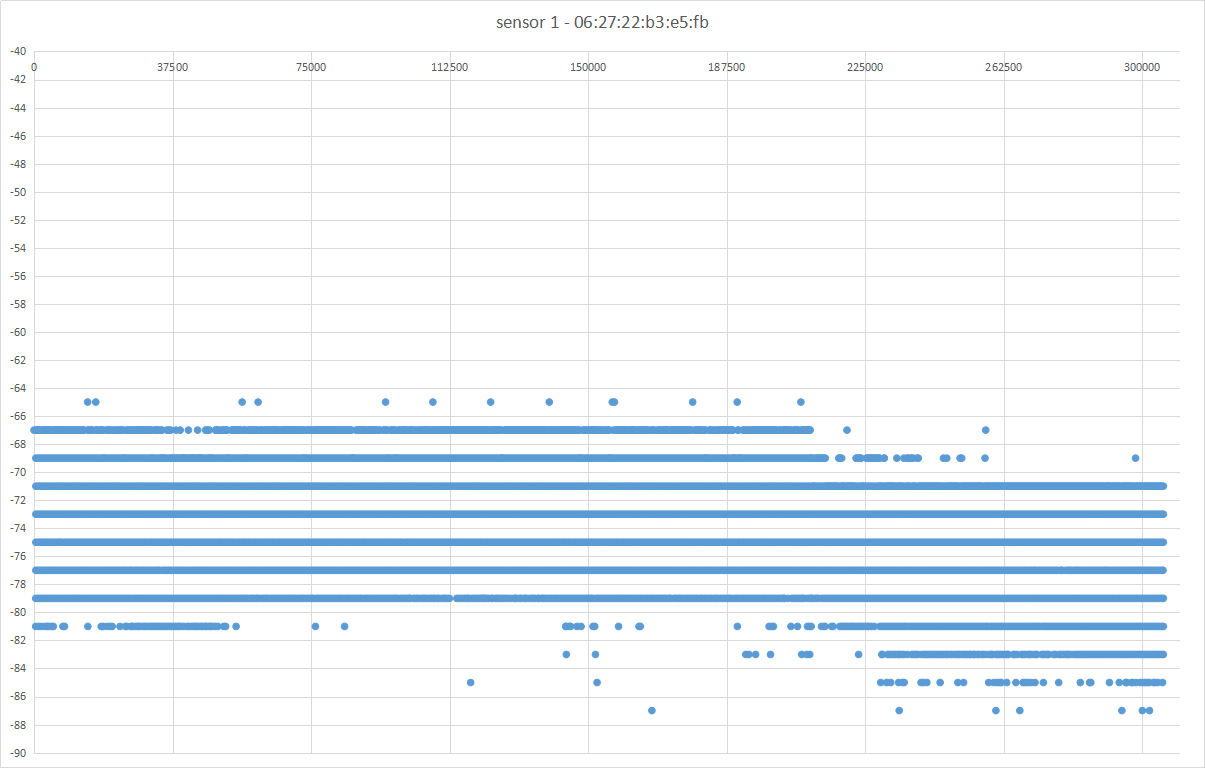
\includegraphics[width=1\textwidth]{060-testes/data-analisis/night-run/062722b3e5fb-sensor-01.png}
		\legend{Fonte: Elaborada pelo autor}
	\end{minipage}
\hfill
	\begin{minipage}{0.49\textwidth}
	\centering
		\caption{\label{fig-062722b3e5fb-s2}Sinal em dBm por pacote capturado - 062722b3e5fb sensor 2}
		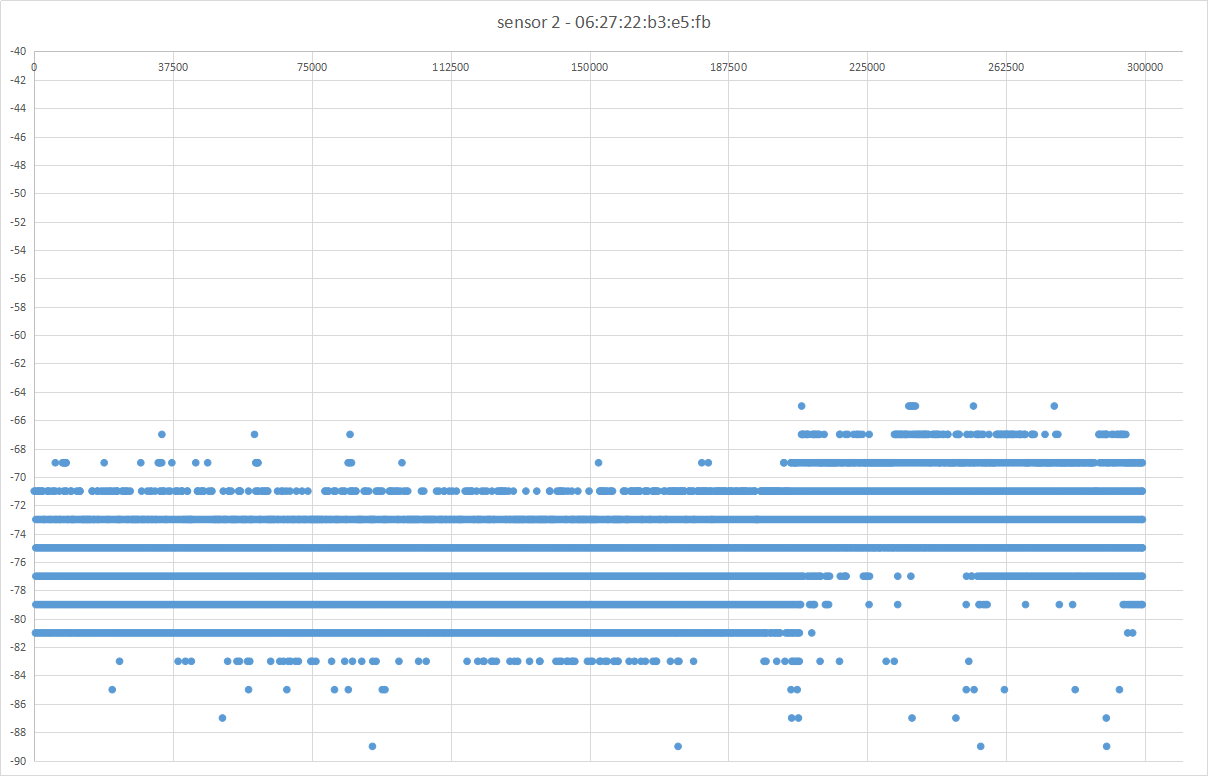
\includegraphics[width=1\textwidth]{060-testes/data-analisis/night-run/062722b3e5fb-sensor-02.png}
		\legend{Fonte: Elaborada pelo autor}
	\end{minipage}
\hfill
	\begin{minipage}{0.49\textwidth}
	\centering
		\caption{\label{fig-062722b3e5fe-s1}Sinal em dBm por pacote capturado - 062722b3e5fe sensor 1}
		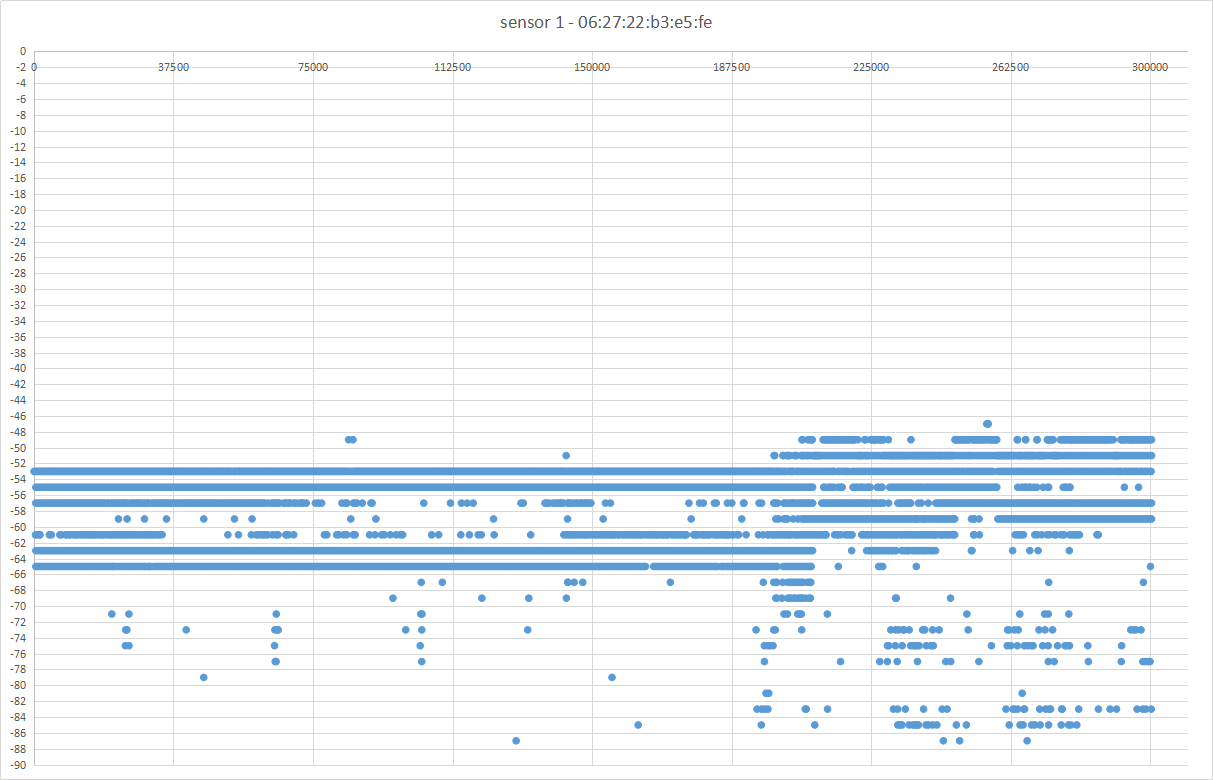
\includegraphics[width=1\textwidth]{060-testes/data-analisis/night-run/062722b3e5fe-sensor-01.png}
		\legend{Fonte: Elaborada pelo autor}
	\end{minipage}
\hfill
	\begin{minipage}{0.49\textwidth}
	\centering
		\caption{\label{fig-062722b3e5fe-s2}Sinal em dBm por pacote capturado - 062722b3e5fe sensor 2}
		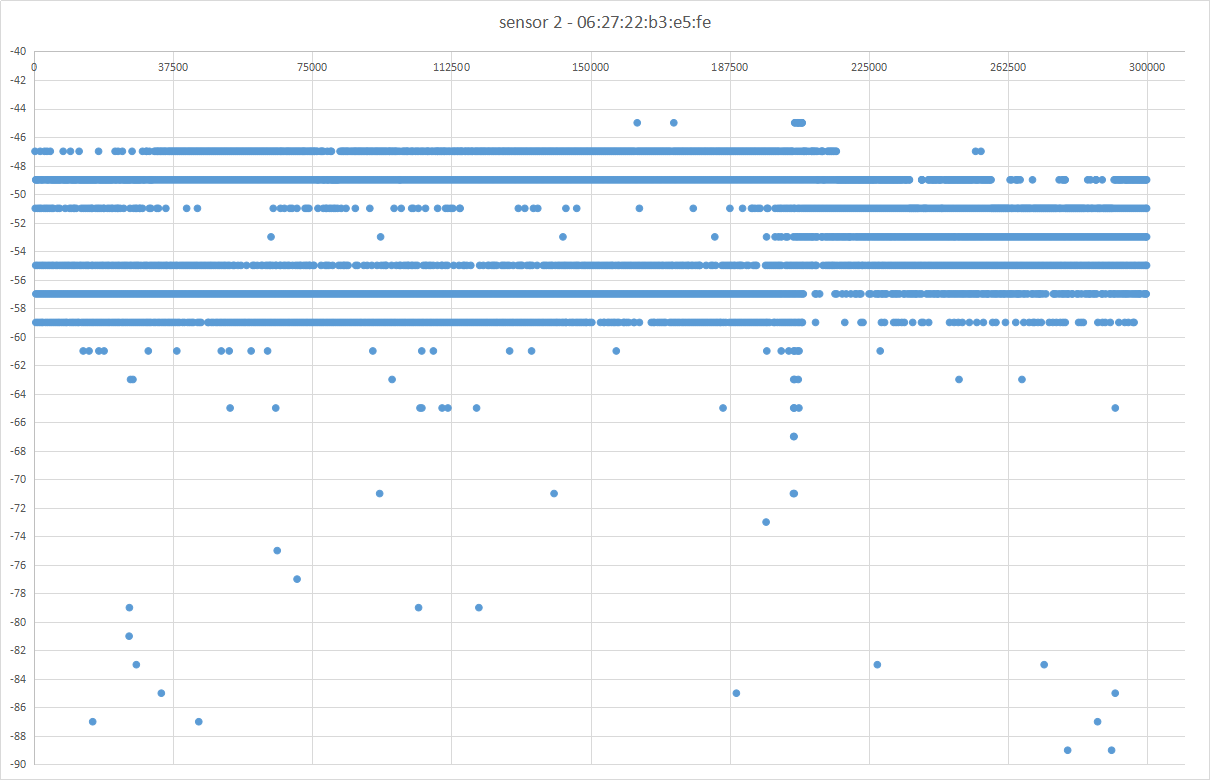
\includegraphics[width=1\textwidth]{060-testes/data-analisis/night-run/062722b3e5fe-sensor-02.png}
		\legend{Fonte: Elaborada pelo autor}
	\end{minipage}
\end{figure}

Imediatamente percebe-se que, apesar da distância ser invariável durate todo o
teste, ela não permaneceu remotamente constante. Nota-se também que o valor
nunca assume valor par. Estas duas características fazem com que o gráfico
seja feito de 7 linhas paralelas ao centro e alguns grupos de pontos ao redor.

Nota-se também uma abrupta mudança no comportamento próximo do pacote 225 000.
Estimou-se que esta mudança é devido ao horário (08:00) em que a universidade
(incluindo o prédio piloto e seus arredores) inicia o seu funcionamento.

Para ter uma visão geral clara da distribuição das potências de sinal calculamos
a média e o desvio padrão para cada um dos casos. Além disso adicionamos o
quanto o desvio padrão representa da média (erro).

\begin{table}[htb]
\IBGEtab{%
\ABNTEXchapterfont {
	\caption{\label{table:ap-pwr-avg}dBm Pontos de acesso - Acumulado 8 horas}%
}
}{%
\begin{tabular}{c|cc|cc}
\toprule
\midrule
AP							& \multicolumn{2}{c}{06:27:22:b3:e5:fe}		&	\multicolumn{2}{c}{06:27:22:b3:e5:fb}	\\
							&	Sensor 1		&	Sensor 2			&	Sensor 1		&	Sensor 2			\\
\midrule
Pacotes						&	300403			&	299864				&	305735			&	299264				\\
\midrule
Média (dBm)					& 	-57.66137822	&	-52.57644132		&	-73.04459417	&	-76.12900984		\\
\midrule
$\sigma$ (Desvio Padrão em dBm)	&	4.746974756		&	3.712407998			&	3.05045545		&	2.889560991			\\
$\sigma$ \%					&	8\%				&	7\%					&	4\%				&	4\%					\\
\midrule
%$3 \times \sigma $			&	14.24092427		&	11.13722399			&	9.151366351		&	8.668682972			\\
%$3 \times \sigma $ \%		&	25\%			&	21\%				&	13\%			&	11\%				\\
%\midrule
\bottomrule
\end{tabular}%
}{%
	\fonte{Produzido pelo autor.}%
}
\end{table}


Em alguns trabalhos podemos
encontrar a equação de FSPL (\emph{Free-space path loss} - perca no caminho em
espaço aberto) que é usualmente utilizada para determinar a potência do sinal
a ser transmitido para que este alcance o seu destinatário.

\begin{equation}
	{\mbox{FSPL(dB)}}=20\log _{{10}}(\text{d})+20\log _{{10}}(\text{f})+92.45
\end{equation}

Na aplicação \emph{Android} \emph{Wifi Distance Calculator} desenvolvida por
\citeonline{Kuik2016} e no trabalho de \citeonline{androidtri} a seguinte
equação é utilizada.

\begin{equation}
	\text{d} = 10 ^{ \frac{1}{20} \left( \text{p} - 20 \times log_{10}\left(\text{f}\right)  + 27.55 \right) } \\
\end{equation}

Onde $d$ é a distância em metros, $p$ é a potência do sinal em $dB$ e $f$
é a frequência do sinal em $MHz$. Como as redes Wi-Fi utilizam canais na região
de 2.4GHz e 5GHz \cite{ieee80211} podemos simplificar a equação e chegar nos
resultados \autoref{eq:2.4ghz} e \autoref{eq:5ghz} respectivamente.

\begin{align}
\text{d}	&= 10 ^{ \frac{1}{20} \left( \text{p} - 20 \times log_{10}\left(\text{2400}\right)  + 27.55 \right) } \nonumber \\
			&= 10 ^{ \frac{1}{20} \left( \text{p} - 40.0542 \right) } \label{eq:2.4ghz}
\end{align}

\begin{align}
\text{d}	&= 10 ^{ \frac{1}{20} \left( \text{p} - 20 \times log_{10}\left(\text{5000}\right)  + 27.55 \right) } \nonumber \\
			&= 10 ^{ \frac{1}{20} \left( \text{p} - 46.4294 \right) } \label{eq:5ghz}
\end{align}

Utilizando a \autoref{eq:2.4ghz} podemos inferir as distâncias entre os sensores
e pontos de acesso a partir da \autoref{table:ap-pwr-avg}. Na
\autoref{table:ap-distance} temos a distância em função da potência $d(p)$
calculada para a potência média ($\overline{dBm}$) e para o erro.


\begin{table}[htb]
\IBGEtab{%
\ABNTEXchapterfont {
	\caption{\label{table:ap-distance}Distância entre os sensores e os Pontos de acesso}%
}
}{%
\begin{tabular}{c|cc|cc}
\toprule
\midrule
AP							& \multicolumn{2}{c|}{06:27:22:b3:e5:fe}		&	\multicolumn{2}{c}{06:27:22:b3:e5:fb}	\\
							&	Sensor 1		&	Sensor 2			&	Sensor 1		&	Sensor 2			\\
\midrule
$d(\overline{dBm})$ metros
							&	7.639569932		&	4.254240777			&	44.89828049		&	64.03987741	\\
\midrule
$d(\overline{dBm} + \sigma)$ metros
							&	13.19525078		&	6.522926214			&	63.78998224		&	89.31585118	\\
$d(\overline{dBm} - \sigma)$ metros
							&	4.423032932		&	2.774608204			&	31.60144461		&	45.91688759	\\
\midrule
Erro acumulado metros		&					&						&					&				\\
$d(\overline{dBm}-\sigma)-d(\overline{dBm}+\sigma)$
							&	8.772217849		&	3.748318009			&	32.18853763		&	43.39896359	\\
\midrule
Erro acumulado em			&					&						&					&				\\
relação a distância (\%)	&	115\%			&	88\%				&	72\%			&	68\%		\\
\midrule
\bottomrule
\end{tabular}%
}{%
	\fonte{Produzido pelo autor.}%
}
\end{table}

A \autoref{table:ap-distance} mostra em sua última linha o erro final encontrado
para a modesta estimativa de uma vez o desvio padrão em relação a distância
calculada a partir do valor de potência médio e o seu tamanho é assombroso.
Esse erro descarta qualquer possíbilidade de associar a potência de sinal a uma
localização geográfica.

Além disso, a definição do padrão IEEE 802.11 inclui que a potência de sinal
utilizada por uma estação para transmissão pode ser variada e a implementação
do método escolhido para a escolha da potência não faz parte do padrão.

\begin{citacao}[english]

	A STA may use any criteria, and in particular any path loss and link margin
	estimates, to dynamically adapt the transmit power for transmissions of an
	MPDU to another STA. The adaptation methods or criteria are beyond the scope
	of this standard. \

	\citeonline[10.8.6,p. 1047]{ieee80211}
\end{citacao}

Esta definição afasta ainda mais a possíbilidade de associação entre o sinal
recebido e a distância calulada através das equações de FSPL.

Em conclusão, esta seção mostra os níveis de erro que são encontrados
utilizando-se somente as equações de FSPL em um ambiente real e justifica o não
uso de valores de geolocalização como um objetivo deste trabalho.
